%=============================================================================
%  SBR 2026 - Brazilian Symposium on Robotics
%  VERSAO DE SUBMISSAO - DOUBLE BLIND - Ingles - max. 6 paginas
%  Camera-ready (15/09/2026): procure pelos blocos "CAMERA-READY".
%
%  >>> VERSAO ANTIGA, ANOTADA <<<
%  Esta e a versao anterior a revisao. Os trechos GRIFADOS EM AMARELO sao os
%  que foram REESCRITOS ou REMOVIDOS em main_corrigido.tex; as marcas [+ ...]
%  em amarelo indicam ONDE material novo foi INSERIDO na versao corrigida.
%  Compare com main_corrigido.tex, onde o texto novo esta grifado.
%
%  Para voltar ao PDF limpo, troque \markchangestrue por \markchangesfalse.
%=============================================================================
\documentclass[conference]{IEEEtran}
\IEEEoverridecommandlockouts

\usepackage[T1]{fontenc}
\usepackage[utf8]{inputenc}
\usepackage{amsmath,amssymb}
\usepackage{graphicx}
\usepackage{booktabs}
\usepackage{multirow}
\usepackage{url}
\usepackage{cite}
\usepackage[hidelinks]{hyperref}

% ---- Marcacao dos trechos alterados na revisao ------------------------------
\usepackage{xcolor}
\usepackage{soul}
\sethlcolor{yellow}
\newif\ifmarkchanges
\markchangestrue          % <<< troque para \markchangesfalse para o PDF limpo
% \chg{...}  = texto ANTIGO que mudou (reescrito ou removido) na versao corrigida
% \ins{...}  = ponto onde a versao corrigida INSERE material novo
\newcommand{\chg}[1]{\ifmarkchanges\hl{#1}\else#1\fi}
\newcommand{\ins}[1]{\ifmarkchanges\hl{\footnotesize[+ #1]}\fi}
% Dentro de \chg, \cite, \ref e matematica inline precisam vir em \mbox{}.
% -----------------------------------------------------------------------------

% Double-blind: impede vazamento de identidade nos metadados do PDF.
\hypersetup{pdftitle={SBR 2026 Submission}, pdfauthor={}, pdfsubject={},
            pdfkeywords={}, pdfcreator={}}

\graphicspath{{figs/}}
\emergencystretch=1em

\begin{document}

\title{Data Drift in a Seq2Seq Model for Robot\\Trajectory Prediction in the RoboCup SSL}

% >>> SUBMISSAO DOUBLE BLIND - MANTENHA ESTE BLOCO <<<
\author{\IEEEauthorblockN{Anonymous Author(s)}
\IEEEauthorblockA{\textit{Affiliation omitted for double-blind review}\\
\textit{Institution omitted}\\
Contact information omitted}}
%
% >>> CAMERA-READY: apague o bloco acima e descomente o modelo abaixo <<<
% \author{
% \IEEEauthorblockN{1\textsuperscript{st} Given Name Surname}
% \IEEEauthorblockA{\textit{dept.} \\ \textit{organization}\\ City, Country \\ email}
% \and ...
% }

\maketitle

% REVISAO: abstract inteiro reescrito (ver main_corrigido.tex).
\begin{abstract}
\chg{Trajectory prediction models are usually reported on a fixed slice of data,
which says little about how long they remain useful. This paper audits a
sequence-to-sequence (seq2seq) predictor for the RoboCup Small Size League
(SSL) that was trained on 2019 world-cup logs and evaluated on the 2021--2025
seasons. The average displacement error (ADE) drifts upward after training,
with an excess of up to \mbox{$+0.73$}\,mm in 2022--2025 on top of a
\mbox{$+3.05$}\,mm jump in the virtual 2021 edition; the Kalman benchmark
degrades even faster, so the neural model's relative advantage grows under
drift. Importance weighting via LSIF attributes 59--72\,\% of the excess ADE to
covariate shift, dominated by tail acceleration; the estimate survives weight
clipping and a relative density-ratio transform, and an independent classifier
two-sample test confirms the shift in every season. Conservative fine-tuning
cuts catastrophic forgetting from 0.82 to 0.46, and a sweep of the elastic
weight consolidation penalty over eight orders of magnitude shows that the
protection comes from the low learning rate rather than from the Fisher term.
Finally, an ADWIN detector calibrated on the error stream under a two-fold
holdout by matches reaches a false-alarm rate of 0.04--0.13 per thousand
trajectories with 9/10 year-folds covered.}
\end{abstract}

\begin{IEEEkeywords}
trajectory prediction, data drift, covariate shift, drift detection,
RoboCup SSL, mobile robots
\end{IEEEkeywords}

%=============================== INTRODUCTION ================================
\section{Introduction}
\label{sec:intro}

Predicting where a robot will be a fraction of a second from now is a routine
requirement in systems with fast dynamics. In the RoboCup Small Size League
(SSL), where six to eleven robots per team move at several meters per second
under centralized control, such predictions feed planning, positioning and
real-time decision making. \ins{o que e a Division A}

The Kalman filter~\cite{kalman} is the traditional benchmark for this task:
cheap, deterministic and easy to tune. \ins{define o termo Kalman-filter
baseline} It also rests on restrictive kinematic
assumptions, namely dynamics that are smooth enough to be captured by a local
linear model. Sequence-to-sequence (seq2seq) networks relax those assumptions
and learn future action patterns directly from logged matches. \ins{cita
Steuernagel e M\'aximo aqui} Better accuracy
on one season, however, is not the same as being usable three seasons later.
\chg{Robots are rebuilt, control stacks are rewritten and playing styles change, so
a model trained on old logs may quietly decay. That is the data drift problem
studied here.}

\chg{The starting point is the seq2seq predictor of Steuernagel and
M\'aximo\mbox{~\cite{seq2seq}}, which remains the reference architecture for
trajectory prediction in the SSL. This paper does not propose a new
architecture. It audits that reference model across seven years of official
world-cup logs and answers four questions:}

\begin{enumerate}
  \item how the error evolves across seasons, at two prediction horizons, and
        how that evolution compares to the \chg{Kalman benchmark};
  \item what fraction of the degradation is explained by covariate shift, and
        which kinematic dimension dominates it;
  \item whether light adaptation recovers accuracy without catastrophic
        forgetting;
  \item whether an online detector can flag the drift with a false-alarm rate
        low enough to trigger retraining.
\end{enumerate}

\ins{paragrafo de outline do artigo}

%============================== RELATED WORK =================================
\section{Related Work}
\label{sec:related}

% REVISAO: secao inteira ampliada e reescrita (ver main_corrigido.tex).
\textbf{Trajectory prediction.}
\chg{The field moved from social pooling between neighboring LSTMs
(Social-LSTM\mbox{~\cite{alahi2016}}) to dynamic graphs with multimodal latent
variables (Trajectron++\mbox{~\cite{salzmann2020}}), agent-aware
transformers\mbox{~\cite{yuan2021}} and diffusion models\mbox{~\cite{gu2022}}.
Within the SSL, Steuernagel and M\'aximo\mbox{~\cite{seq2seq}} applied an
attention-based seq2seq model at the same horizons used here, and it is the
direct baseline of this work. All of these evaluations use fixed data splits;
temporal stability across seasons has received far less attention.}

\textbf{\chg{Drift and online detection.}}
Gama et al.~\cite{gama2014} separate virtual drift, a change in $p(x)$, from
real drift, a change in $p(y|x)$. \ins{por que a distincao importa na pratica}
\chg{Detectors are usually error-based, such as
ADWIN\mbox{~\cite{adwin}} and Page--Hinkley\mbox{~\cite{page_hinkley}}, or
data-based, such as KSWIN\mbox{~\cite{kswin}}.} Lu et al.~\cite{lu2019} argue
that calibrating the
false-alarm rate is what makes a detector trustworthy in production, and that
requirement is taken here as the design constraint of
Section~\ref{sec:detection}. \ins{EWC e o trade-off estabilidade--plasticidade}

\textbf{Covariate shift.}
\chg{Direct density-ratio estimation through LSIF or
KLIEP\mbox{~\cite{kliep,kanamori2009,sugiyama_book}} corrects covariate shift
without retraining. RuLSIF\mbox{~\cite{yamada2013}} is the relative-ratio
variant with bounded weights, and the classifier two-sample
test\mbox{~\cite{lopezpaz2017}} detects shift without assuming a functional
form.} LSIF is used here as the main estimator,
with the other two serving as robustness checks.

%================================= METHOD ====================================
\section{Data and Model}
\label{sec:method}

\textbf{Data.}
The study uses official logs from the 2019--2025 \chg{world cups}, excluding
\chg{2020, when no in-person championship was held: six Division~A matches per
year, 36 matches in total,} captured at 60\,Hz. The 2021 edition was played
entirely in simulation \chg{after the pandemic}. It is kept in the descriptive
analyses because it carries the largest distribution jump of the period
($+3.05$\,mm of excess ADE), but part of that jump plausibly reflects the
\chg{simulation-to-reality gap} rather than organic drift, so it is reported
separately throughout and excluded from the adaptation experiments of
Section~\ref{sec:adaptation}.
Consolidating a model against an anomalous simulated season would contaminate
the old regime with a distribution that no longer describes the league.
\chg{League composition is constant across the logs, so the observed excess
cannot be attributed to a change of division.} Per-trajectory analyses sample
8\,000 windows per match, yielding a temporally ordered stream of 288\,000
trajectories, 48\,000 per year. The 2019 baseline uses all six matches of the
year: a sensitivity sweep shows that a single reference match puts
$\mathrm{ADE}_{2019}$ anywhere between 4.53 and 6.20\,mm, enough to flip the
sign of the excess in four of the five remaining years.\footnote{Code and
processed data will be released upon acceptance; the link is omitted for
double-blind review.}

\textbf{Model and benchmark.}
\chg{The replicated architecture follows\mbox{~\cite{seq2seq}}}: a 128-unit LSTM
encoder, \chg{additive Bahdanau attention\mbox{~\cite{bahdanau}}} and an
autoregressive LSTM decoder
without teacher forcing, trained with Adam~\cite{adam} at an initial learning
rate of $10^{-3}$, batch size 1024 and early stopping. Each input step carries
six normalized variables: \chg{position \mbox{$x,y$}, velocity
\mbox{$v_x,v_y$} and orientation \mbox{$\sin\psi$}, \mbox{$\cos\psi$}.}
\ins{como e feita a normalizacao} One detail matters for the drift analysis:
the target
lives in the space of normalized incremental velocities, and the future
position is reconstructed from the last observed state. The model therefore
predicts accumulated dynamics, which makes it directly sensitive to changes in
the velocity and acceleration distributions. \chg{The kinematic comparator is
the constant-velocity predictor corresponding to the steady state of a Kalman
filter\mbox{~\cite{kalman}}: deterministic, parameter-free and identical in
every season, so any degradation on its side reflects robot behavior alone.}

\textbf{Metric.}
For $N$ trajectories and horizon $H$, the average displacement error is
\begin{equation}\label{eq:ade}
\mathrm{ADE} = \frac{1}{NH} \sum_{i=1}^{N}\sum_{t=1}^{H}
\left\lVert \hat{p}_{i,t} - p_{i,t} \right\rVert_2 ,
\end{equation}
\chg{where \mbox{$\hat{p}_{i,t}$} is the predicted position and
\mbox{$p_{i,t}$} the observed one.}
Descriptive results cover the $30 \rightarrow 15$ and $60 \rightarrow 30$
horizons; \ins{explica a notacao $a \rightarrow b$} the mechanism and detection
analyses use $30 \rightarrow 15$.

%============================== DEGRADATION ==================================
\section{Temporal Degradation}
\label{sec:degradation}

\begin{figure}[!t]
  \centering
  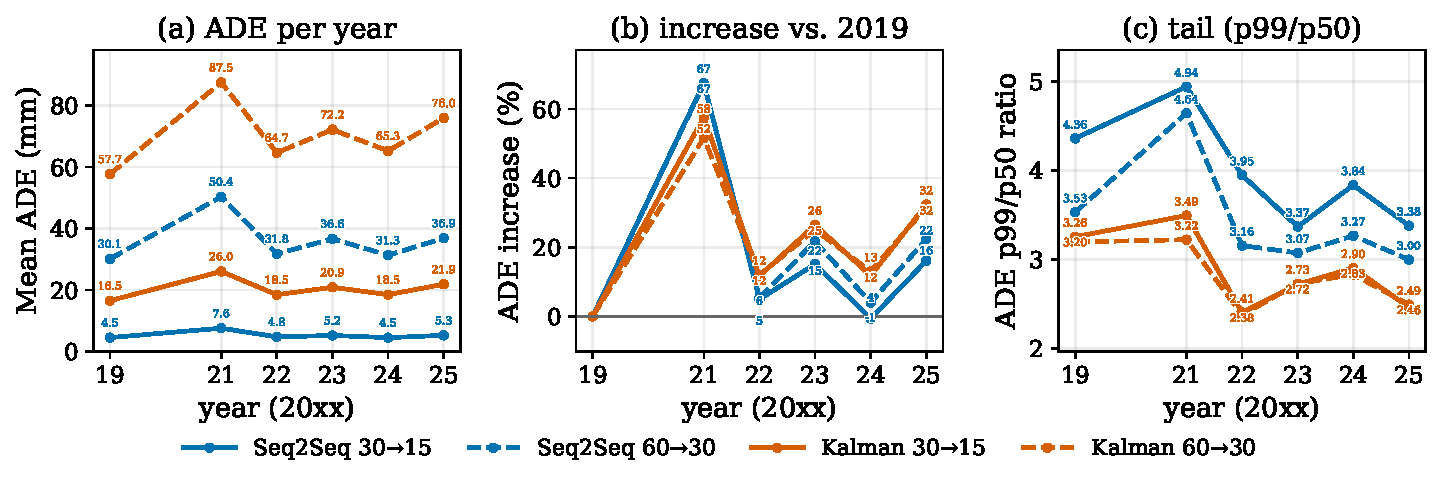
\includegraphics[width=\columnwidth]{fig_degradacao_en}
  \caption{Temporal degradation (color = model, line style = horizon).
  (a) Mean ADE per year. (b) Percentage increase in ADE relative to 2019.
  (c) $\mathrm{p99}/\mathrm{p50}$ ratio of the per-trajectory ADE: the 2021
  jump is a tail effect ($4.36 \to 4.94$), whereas in 2022--2025 the ratio
  falls below baseline while the median rises by about 25\,\%.}
  \label{fig:degradation}
\end{figure}

Fig.~\ref{fig:degradation} summarizes three descriptive findings.

\textbf{The seq2seq model degrades outside its training distribution.}
\chg{ADE grows in every post-2019 season, and the excess trends upward through
2022--2025, from \mbox{$+0.23$}\,mm in 2022 to \mbox{$+0.73$}\,mm in 2025 at
the \mbox{$30 \rightarrow 15$} horizon, with 2024 close to zero. The virtual
2021 season stands apart at \mbox{$+67\,\%$} for the reason given in
Section~\mbox{\ref{sec:method}}.}
The pattern repeats at both horizons.

\textbf{\chg{The Kalman benchmark degrades more.}}
Its relative error growth exceeds that of the seq2seq model in nearly every
season. \ins{o filtro de Kalman nao e treinado} The right reading is not that
the neural model is stable, since its absolute error also
grows, but that the kinematic \chg{benchmark} is even more sensitive to the
regime change, so the comparative advantage of learning widens under drift.

\textbf{The new regime enters through the tail, then spreads.}
The $\mathrm{p99}/\mathrm{p50}$ ratio rises only at the 2021 jump
($4.36 \to 4.94$), when the model fails disproportionately on a tail of
trajectories. In the following seasons the ratio drops below baseline, to
$3.4$--$4.0$: the median climbs about 25\,\% up to 2025 while the 99th
percentile stays flat. Behavior that used to be rare has become ordinary, and
the gradual degradation now sits in the body of the distribution.

\begin{figure}[!t]
  \centering
  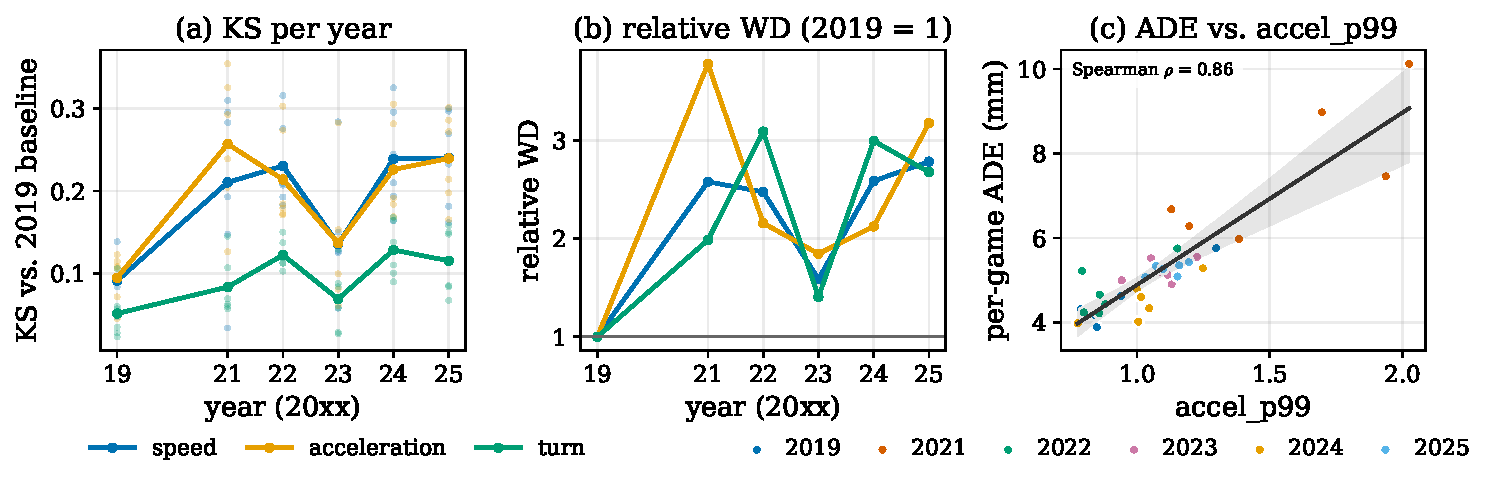
\includegraphics[width=\columnwidth]{fig_drift_cinematico_en}
  \caption{Kinematic drift. \protect\chg{(a) KS statistic per year against the
  2019 baseline (lines: annual mean; dots: matches). (b) Wasserstein distance
  indexed to the 2019 level.} (c) Mean ADE per match against the match's
  \texttt{accel\_p99}, with a regression line and a 95\,\% bootstrap band.}
  \label{fig:kinematic}
\end{figure}

Measuring the input side directly confirms the picture
(Fig.~\ref{fig:kinematic}). \chg{Against the 2019 baseline, both the
Kolmogorov--Smirnov statistic and the Wasserstein distance show clear and
persistent shifts in velocity and acceleration, while turn rate moves much
less.} At match level, ADE grows almost monotonically with the match's tail
acceleration (\texttt{accel\_p99}, Spearman $\rho = 0.86$): the more aggressive
the match, the worse the model does, regardless of the season it belongs to.

%================================= IW ========================================
\section{How Much of It Is Covariate Shift?}
\label{sec:iw}

The joint distribution factors as $p(x,y) = p(y|x)\,p(x)$~\cite{gama2014}.
Covariate shift changes only $p(x)$ and can be corrected by reweighting old
samples, with no retraining; concept drift changes $p(y|x)$ and requires fresh
labels. Telling them apart decides whether the cheap fix is available.

LSIF~\cite{kliep,kanamori2009,sugiyama_book} estimates the density ratio
$\hat{w}(x) = p_{\text{target}}(x)/p_{2019}(x)$ directly as a combination of
Gaussian kernels,\ins{define os coeficientes $\boldsymbol\alpha$}
\begin{equation}\label{eq:lsif}
\min_{\boldsymbol\alpha \geq 0}\;
\tfrac{1}{2}\,\mathbb{E}_{p_{2019}}[\hat{w}(x)^2] -
\mathbb{E}_{p_{\text{target}}}[\hat{w}(x)] + \lambda\|\boldsymbol\alpha\|^2 ,
\end{equation}
with $x \in \mathbb{R}^{8}$ collecting the kinematic features of each observed
window: mean, p90 and p99 of speed and acceleration, plus mean and p90 of turn
rate, clipped at the 99.5th percentile of the pool and passed through
$\log(1+\cdot)$. Stability is monitored by the effective sample size
$\mathrm{ESS} = (\sum_i \hat{w}_i)^2/(n\sum_i \hat{w}_i^2)$, with the usual
$\mathrm{ESS} > 0.5$ rule of thumb~\cite{sugiyama_book}. The weighted error and
the recovered fraction of the excess are
\begin{equation}\label{eq:recovery}
\mathrm{ADE}_{\mathrm{IW}} = \frac{\sum_i \hat{w}(x_i)\,e_i}{\sum_i \hat{w}(x_i)},
\quad
\mathrm{rec.} = \frac{\mathrm{ADE}_y - \mathrm{ADE}_{\mathrm{IW}}}
                     {\mathrm{ADE}_y - \mathrm{ADE}_{2019}} .
\end{equation}
\ins{define $e_i$ e $\mathrm{ADE}_y$}
A recovery of 100\,\% would mean pure covariate shift, and 0\,\% pure concept
drift.

\begin{table}[!t]
\centering
\caption{Importance-weighting decomposition (LSIF) with block bootstrap by
match ($n_{\text{boot}} = 2000$, 6 blocks per year). Baseline
$\mathrm{ADE}_{2019} = 4.53$\,mm; corr.\ $= \mathrm{ADE}_y -
\mathrm{ADE}_{\mathrm{IW}}$. 2024 has negative excess and is excluded from the
recovery column. All classifier tests give $p < 10^{-3}$ by permutation.
$^{\dagger}$2022 has a small excess (0.23\,mm), so the percentage should be
read with care.}
\label{tab:iw}
\footnotesize
\setlength{\tabcolsep}{3pt}
\begin{tabular}{@{}rrrlll@{}}
\toprule
\textbf{Year} & \textbf{ADE$_y$} & \textbf{ADE$_{\mathrm{IW}}$}
 & \textbf{rec.\ (\%) [95\,\% CI]} & \textbf{corr.\ (mm)} & \textbf{AUC} \\
\midrule
2021 & 7.58 & 5.70 & 61.6 $[43.7;\,79.3]$          & 1.88 $[1.33;\,2.42]$ & 0.754 \\
2022 & 4.75 & 4.62 & 59.0 $[9.2;\,115.2]^{\dagger}$ & 0.13 $[0.02;\,0.26]$ & 0.647 \\
2023 & 5.21 & 4.72 & 71.8 $[43.8;\,109.2]$          & 0.49 $[0.30;\,0.75]$ & 0.657 \\
2024 & 4.50 & 4.24 & ---                            & ---                  & 0.612 \\
2025 & 5.26 & 4.75 & 69.3 $[57.2;\,79.0]$           & 0.51 $[0.42;\,0.58]$ & 0.710 \\
\bottomrule
\end{tabular}
\end{table}

\textbf{Robustness.}
Any quantitative claim here depends on the weights behaving well under the
heavy tail of \texttt{accel\_p99}. Three checks support them. First, the
weights are bounded: $\max_i \hat{w}_i \in [2.9;\,4.4]$ in every season, and
the ESS of $0.58$--$0.73$ comes from the near-zero mass assigned to the new
regime, which is the correct mechanism for reconstructing 2019, not from
extreme weights (the top 1\,\% of trajectories carries only 3--4\,\% of the
mass). Second, capping the weights at $c \in \{1.5,\ldots,50\}$ leaves recovery
saturated from $c \approx 3$ onward. Third, applying the RuLSIF relative-ratio
transform $\hat{w}/(\alpha\hat{w}+1-\alpha)$ with $\alpha = 0.1$ keeps recovery
at 59--65\,\%. Fitting RuLSIF directly was tested and discarded: in this
configuration it returns nearly uniform weights ($\mathrm{ESS} \geq 0.94$) and
underestimates recovery at 9--23\,\%, an artifact of the fit rather than of the
estimand, as the two previous checks show.

\textbf{Reading.}
Table~\ref{tab:iw} places LSIF recovery at 59--72\,\% in the years with a
positive excess, with confidence intervals excluding zero. The stronger
statement is on the absolute correction, whose lower bound stays positive even
in 2022 ($\geq 0.02$\,mm): reweighting moves the error toward the 2019 level by
an amount distinguishable from zero with only six bootstrap blocks. The
classifier two-sample test agrees, separating each season from 2019 with
$\mathrm{AUC} \in [0.61;\,0.75]$ and ranking the seasons by severity in the
same order, without estimating any density ratio. The unrecovered 30--40\,\% is
residual concept drift plus sampling noise.

\begin{table}[!t]
\centering
\caption{Marginal recovery per feature (LSIF refitted on one feature at a
time), for the three seasons with a significant excess.}
\label{tab:iwfeat}
\footnotesize
\begin{tabular}{lcccc}
\toprule
\textbf{Feature} & \textbf{2021 (\%)} & \textbf{2023 (\%)} & \textbf{2025 (\%)}
 & \textbf{mean ESS} \\
\midrule
\texttt{accel\_p99}  & \textbf{57.1} & 52.6 & 51.7 & 0.55 \\
\texttt{accel\_p90}  & 54.0          & 51.3 & 51.1 & 0.57 \\
\texttt{accel\_mean} & 43.0          & 47.0 & 49.5 & 0.68 \\
\texttt{speed\_p99}  & 17.2          & 36.1 & 40.1 & 0.84 \\
\texttt{speed\_p90}  & 15.8          & 34.4 & 38.0 & 0.85 \\
\texttt{speed\_mean} &  7.9          & 24.7 & 27.4 & 0.91 \\
\texttt{turn\_p90}   &  3.9          &  0.2 &  0.0 & 0.97 \\
\texttt{turn\_mean}  &  5.3          &  0.9 &  0.0 & 0.96 \\
\bottomrule
\end{tabular}
\end{table}

Refitting LSIF on one feature at a time makes the mechanism concrete
(Table~\ref{tab:iwfeat}). Tail acceleration leads consistently, followed
closely by \texttt{accel\_p90}; speed features recover far less, and turn-rate
features are essentially inert, below 5\,\% in every season. The ranking is
stable across seasons: the league has adopted more aggressive acceleration
profiles, and that is the main vector of degradation. The ESS column moves the
other way, as it should: the features that shifted the most are the ones whose
reweighting costs the most effective sample.

%============================== ADAPTATION ===================================
\section{Adaptation}
\label{sec:adaptation}

Since the excess is mostly covariate, four families of adaptation strategies
were compared under one conservative protocol: old regime $=$ 2019, new data
$=$ 2022--2025 (500 trajectories per match, 2021 excluded as an outlier),
frozen encoder, two trainable decoder layers, $\mathrm{lr} = 10^{-5}$ and five
epochs. Forgetting is measured by \texttt{cat\_ratio}, the fraction of old-regime
trajectories that get worse after the update. Table~\ref{tab:adapt} collects
the results.

\begin{table}[!t]
\centering
\caption{Adaptation strategies under the common conservative protocol. The
unadapted model scores 4.584\,mm on the old regime and 4.965\,mm on the new
data. EWC reports the median of the $\lambda \in [50;\,10^7]$ plateau. The
last three rows are driven by the covariate diagnosis.}
\label{tab:adapt}
\footnotesize
\setlength{\tabcolsep}{4pt}
\begin{tabular}{@{}lccc@{}}
\toprule
\multirow{2}{*}{\textbf{Strategy}} & \multirow{2}{*}{\textbf{\texttt{cat\_ratio}} $\downarrow$}
 & \multicolumn{2}{c@{}}{\textbf{ADE (mm)}} \\
\cmidrule(l){3-4}
 & & \textbf{old} & \textbf{new} \\
\midrule
Conservative FT ($r=0$)     & 0.457          & 4.480          & 4.762 \\
EWC ($\lambda$ plateau)     & 0.457          & 4.481          & 4.817 \\
Uniform replay ($r=0.5$)    & 0.438          & 4.439          & \textbf{4.760} \\
\midrule
Importance-weighted replay  & \textbf{0.417} & \textbf{4.404} & 4.761 \\
Acceleration-selective FT   & 0.467          & 4.526          & 4.811 \\
Selective $+$ IW replay     & 0.449          & 4.441          & 4.800 \\
\bottomrule
\end{tabular}
\end{table}

Naive fine-tuning is destructive: without the conservative protocol,
\texttt{cat\_ratio} reaches 0.82 after a single epoch. Elastic weight
consolidation~\cite{kirkpatrick2017} is the standard remedy, adding
$\frac{\lambda}{2}\sum_i F_i(\theta_i - \theta^{*}_i)^2$ \chg{with
\mbox{$F_i$} the diagonal Fisher information.} The finding here is that the
Fisher term does nothing: sweeping $\lambda \in \{0, 50, \ldots, 10^7\}$ leaves
\texttt{cat\_ratio} pinned near 0.46 across eight orders of magnitude, because
the diagonal is numerically tiny ($F_i \approx 10^{-7}$), as expected from an
already converged decoder. What protects the old regime is the small learning
rate and the frozen encoder.

Mixing a replay buffer of original data into the update, at a replay-to-new
ratio $r = 0.5$, improves all three metrics at once, pushing \texttt{cat\_ratio}
below the no-replay control and reaching the lowest ADE on new data in the
table. The gain is modest, since the conservative schedule already limits
forgetting, but it is consistent and essentially free.

\begin{figure}[!t]
  \centering
  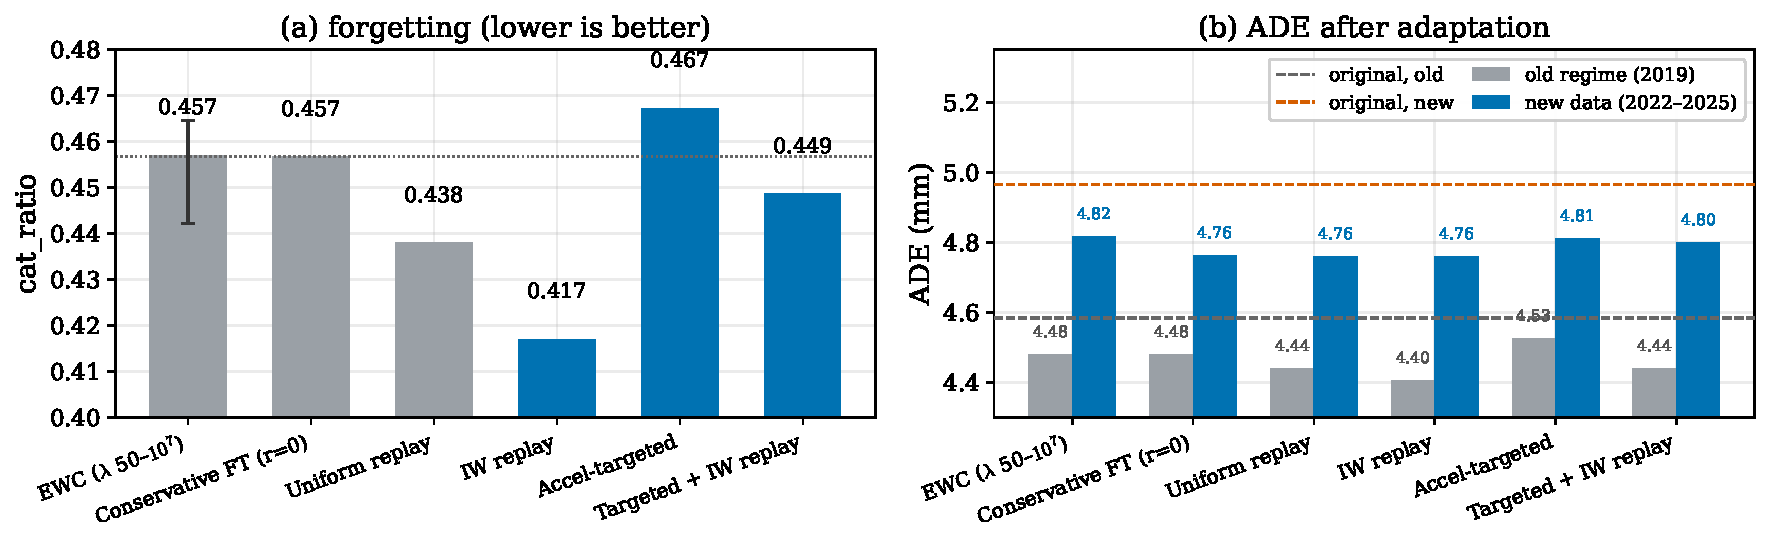
\includegraphics[width=\columnwidth]{fig_finetune_en}
  \caption{Adaptation strategies under the same protocol (blue: variants driven
  by the covariate/acceleration diagnosis). (a) Forgetting, with the error bar
  showing the EWC $\lambda$ plateau and the dotted line the no-replay control.
  (b) ADE after adaptation on both regimes, with the unadapted model as
  reference (dashed lines).}
  \label{fig:finetune}
\end{figure}

Steering adaptation by the covariate diagnosis gives a more interesting split
(Fig.~\ref{fig:finetune}).
Sampling the replay buffer proportionally to $\hat{w}(x)$ helps: it reaches the
lowest \texttt{cat\_ratio} (0.417) and the lowest old-regime ADE in the table,
though by a small margin on a single seed. Hard selection hurts. Fine-tuning
restricted to the top 50\,\% of new data by tail acceleration, exactly the
region where $p(x)$ moved, produces the worst forgetting of all six rows
(0.467), above even the control. The tail is the subset farthest from the 2019
regime, so training only on it displaces the weights more; the unchanged body
of the distribution, which hard selection throws away, acts as an implicit
anchor. Reweighting preserves that anchor and merely emphasizes the relevant
tail. The covariate diagnosis is therefore useful for monitoring, for
explaining the excess and for weighting replay, but not for discarding data.

%============================== DETECTION ====================================
\section{Online Detection}
\label{sec:detection}

The operational question is whether drift can be flagged automatically on the
288\,k-trajectory stream. A detector is judged by three quantities~\cite{lu2019}:
$\mathrm{FAR}_{2019}$, the alarms per thousand trajectories in the training
year, where no drift exists \ins{e todo alarme e falso} (admissibility ceiling
0.20/1k); coverage, the number of 2021--2025 seasons with at least one alarm;
and latency after each
year boundary. To avoid tuning and reporting on the same data, calibration runs
under a two-fold cross-validation by matches: half the matches of each year
select the ADWIN~\cite{adwin} configuration out of a 96-point grid, and the
untouched half is evaluated once. All figures below are out of sample.

Local robust normalization of the per-trajectory signal, by median and MAD over
a 200-trajectory window, is what makes the detector viable at all. On the raw
signal no configuration in the grid is admissible in either fold, and the 21
conventional smoothers tested (moving averages, EWMA, Holt, Savitzky--Golay)
all increase FAR by injecting the autocorrelation that ADWIN assumes away. On
the normalized ADE the winning family is stable across folds
($\delta = 10^{-4}$, windows 1000/5000), giving $\mathrm{FAR}_{2019}$ of
0.042/1k with 5/5 coverage in fold~A and 0.125/1k with 4/5 in fold~B, at a
latency of 0.2 to 1.5 matches. The holdout does more than add confidence here; it changes what one would
deploy. The configuration that in-sample selection picks keeps
$\mathrm{FAR} \approx 0$ and then covers only 2--3 of 5 seasons out of sample.

The diagnosis of Section~\ref{sec:iw} also buys a second monitoring channel.
Because the shift is dominated by tail acceleration, the features of the
observed window carry the drift signal without running the model and without
waiting for the 15 future steps that ADE requires. Applying the same protocol
to four kinematic signals reproduces the ranking of the per-feature
decomposition, with \texttt{accel\_p95} ahead
($\mathrm{FAR} = 0.25$--$0.29$/1k, 5/5 coverage in both folds).\footnote{p95
rather than the dominant p99, because the observed window holds only 29
acceleration samples.} No single feature is admissible on its own, since
kinematics vary naturally within 2019, but the acceleration channel fires
before the error channel in 8 of 10 year-folds, which is enough for a watch
layer. At the other extreme, the conjunction of the two alarms within a
coincidence window of 200 trajectories drives observed false alarms to zero in
both folds, at the cost of coverage (2--3 of 5).

\begin{table}[!t]
\centering
\caption{Layered detection architecture, with metrics on the test split of
each fold (A/B). All signals use robust normalization with $w = 200$; each
detector is configured per fold during calibration.}
\label{tab:detection}
\footnotesize
\setlength{\tabcolsep}{3pt}
\begin{tabular}{@{}llccl@{}}
\toprule
\textbf{Layer} & \textbf{Signal} & \textbf{FAR/1k (A/B)} & \textbf{Cov.}
 & \textbf{Action} \\
\midrule
Primary      & seq2seq ADE          & 0.042 / 0.125 & 5/5, 4/5 & retrain \\
Watch        & \texttt{accel\_p95}  & 0.292 / 0.250 & 5/5, 5/5 & monitor \\
Confirmation & AND(ADE, accel)      & 0.000 / 0.000 & 3/5, 2/5 & confirm \\
\midrule
Corroborator & \chg{Kalman} ADE     & 0.167 / 0.083 & 5/5, 5/5 & redundancy \\
\bottomrule
\end{tabular}
\end{table}

Table~\ref{tab:detection} summarizes the resulting three-layer architecture.
Two caveats and one negative result deserve mention. Per-trajectory FAR assumes
approximately independent trajectories within 2019, and the serial correlation
is real ($\rho_1 = 0.54$); a permutation test shows the violation is
conservative, since shuffling trajectories within matches drives false alarms
to zero in all 200 replicates. Among alternatives, Page--Hinkley~\cite{page_hinkley}
aggregated over windows achieves $\mathrm{FAR} = 0$ but only detects the abrupt
2021 jump, and KSWIN~\cite{kswin} is inadmissible in every configuration
($\mathrm{FAR} \geq 0.438$/1k). The negative result is structural: combining
detectors that run at different time scales is unworkable, because the closest
pair of alarms is 214 trajectories apart, beyond any usable coincidence window.
Aligning the scales fixes it, which is how the confirmation layer above was
obtained.

%============================== CONCLUSION ===================================
% REVISAO: titulo alterado para "Conclusions and Future Work" na versao
% corrigida (nao ha como grifar dentro de \section: o argumento e movel).
\section{Conclusion}
\label{sec:conclusion}

A seq2seq trajectory predictor for the SSL loses accuracy as the league moves
away from its training season. The loss is gradual, it is measurable, and most
of it can be traced to a specific change in the input distribution. Excess ADE
trends upward through 2022--2025 \chg{on top of the jump in the virtual 2021
edition, while the Kalman benchmark degrades faster still.}
Between 59 and 72\,\% of that excess is recovered by importance weighting, an
estimate robust to weight clipping and to the relative-ratio transform and
corroborated by an independent classifier test, with tail acceleration as the
dominant vector.

On the response side, light adaptation keeps forgetting under control
(\texttt{cat\_ratio} from 0.82 to 0.46), EWC turns out to be inert over eight
orders of magnitude of $\lambda$, and a replay buffer improves forgetting and
adaptation at the same time, with the optimum at importance-weighted replay.
Hard selection by the drifting tail backfires. On the operational side, ADWIN
over a robustly normalized error stream reaches a false-alarm rate of
0.04--0.13 per thousand trajectories out of sample with 9/10 year-folds
covered, and the same diagnosis yields a model-free acceleration channel that
anticipates the error alarm in 8 of 10 year-folds.

% REVISAO: paragrafo removido daqui e movido para a Introducao (delimitar a
% contribuicao e assunto de Introducao, nao de Conclusao).
\chg{Relative to\mbox{~\cite{seq2seq}}, the contribution is a shift of question:
not whether the seq2seq model beats the kinematic benchmark on a fixed split,
but how that advantage evolves as the distribution drifts away from the
training season, and what can be done about it.}

Several limitations bound these conclusions. Only Division~A appears in the
logs. Six matches per season keep the block confidence intervals wide, and the
Wilson intervals of the holdout cross the admissibility ceiling, so claiming
admissibility at 95\,\% confidence would require more 2019 matches. ADE is
single-mode and would have to give way to
$\text{min-ADE}_K$~\cite{salzmann2020,yuan2021} for multimodal predictors.
Robust normalization assumes gradual drift and would absorb part of an abrupt
change. The residual concept-drift fraction is not isolated per feature and may
hide covariate shift in unmeasured dimensions. Finally, the 2021 season was
played in simulation, so its error jump mixes the
\chg{simulation-to-reality gap} with seasonal drift, and the gradual-trend
conclusions rest on 2022--2025.
Deeper adaptation, retraining the encoder with an importance-weighted replay
buffer, is the natural next step.

%===================== ACKNOWLEDGMENT (CAMERA-READY ONLY) ====================
% !!! NAO INCLUIR NA SUBMISSAO DOUBLE-BLIND !!!
% \section*{Acknowledgment}
% The authors thank <agencia> for support under <programa/numero>.

\bibliographystyle{IEEEtran}
\bibliography{references}

\end{document}
